% !TEX root = ../../defense.tex

\section{Orbital Transfers}

\begin{frame} \label{slide:lowthrust_vehicles}%-----------------------------%
\frametitle{Low thrust vehicles} % electric propulsion
\begin{itemize}
    \item Low thrust orbital transfers offer increased mission oportunities
    \begin{itemize}
        \item Electric propulsion is increasing in capability
        \item Offers much higher specific impulse than chemical engines 
        \item Requires much longer operating periods for maneuvers 
        \item Enables long duration missions with frequent thrusting
    \end{itemize}
\end{itemize}

\begin{center}
    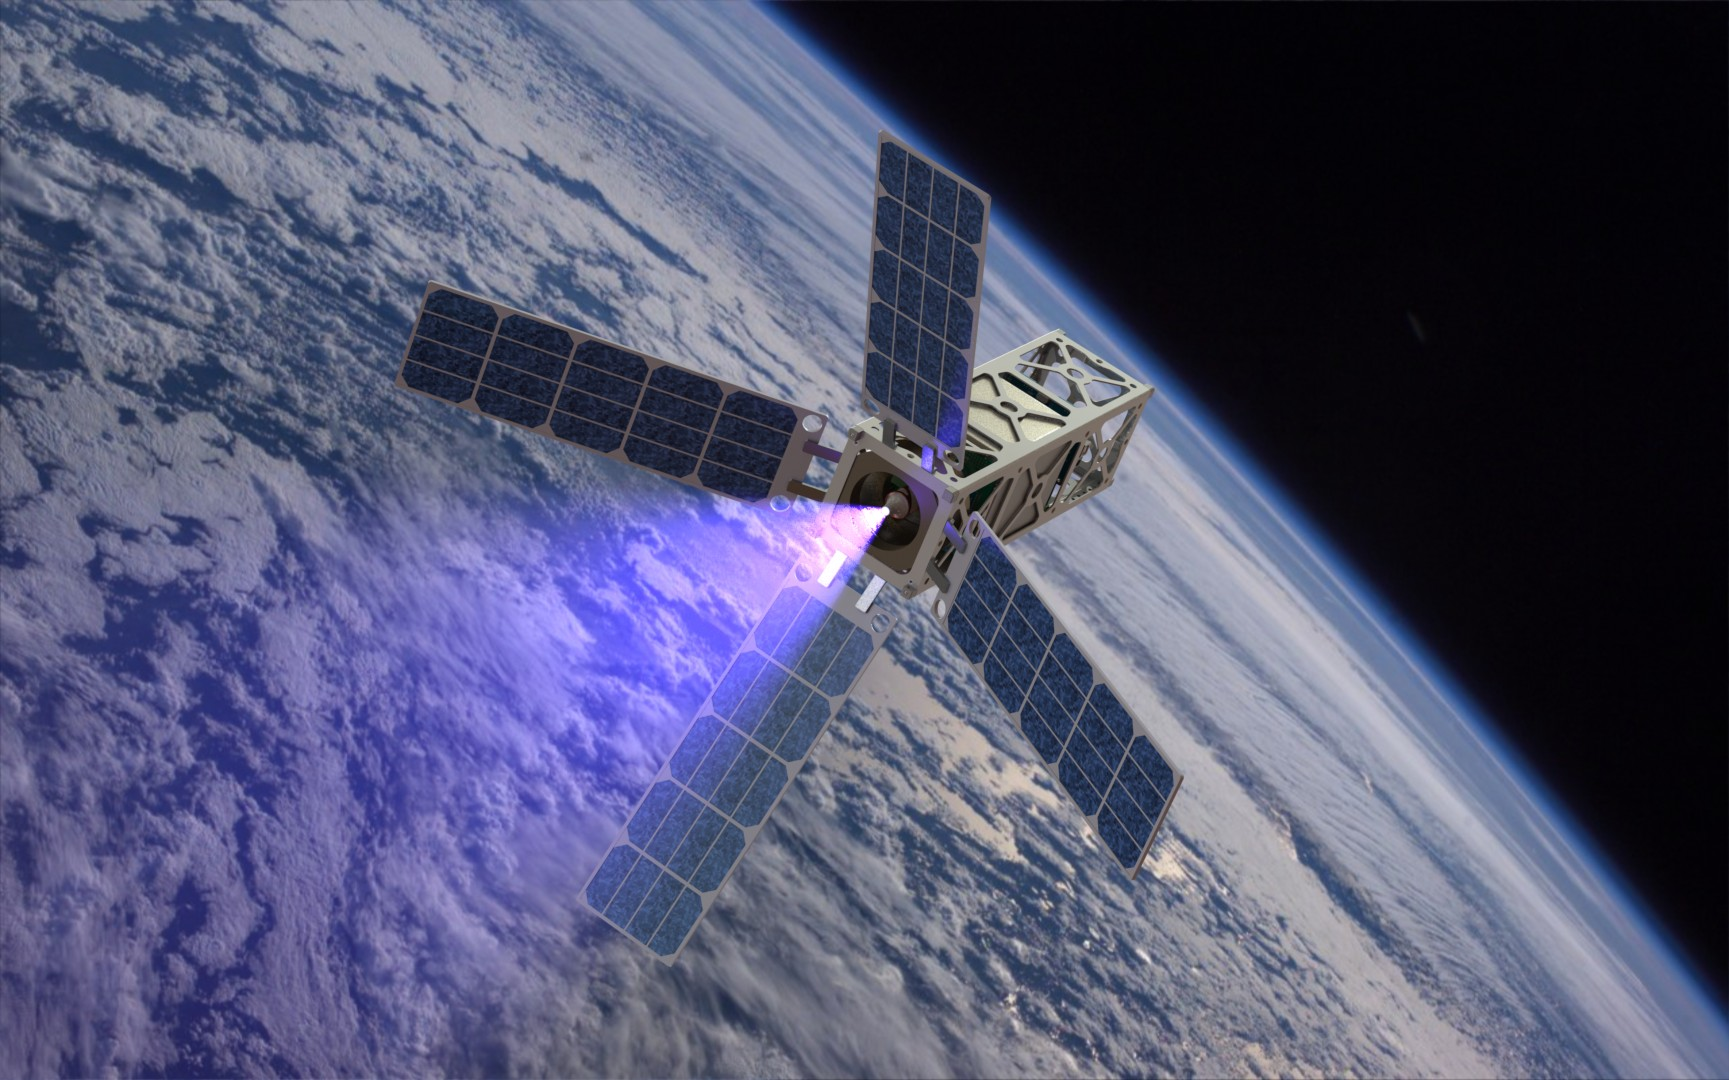
\includegraphics[height=0.4\textheight,width=0.5\textwidth,keepaspectratio]{figures/defense/patriot_plume.jpg}
    ~
    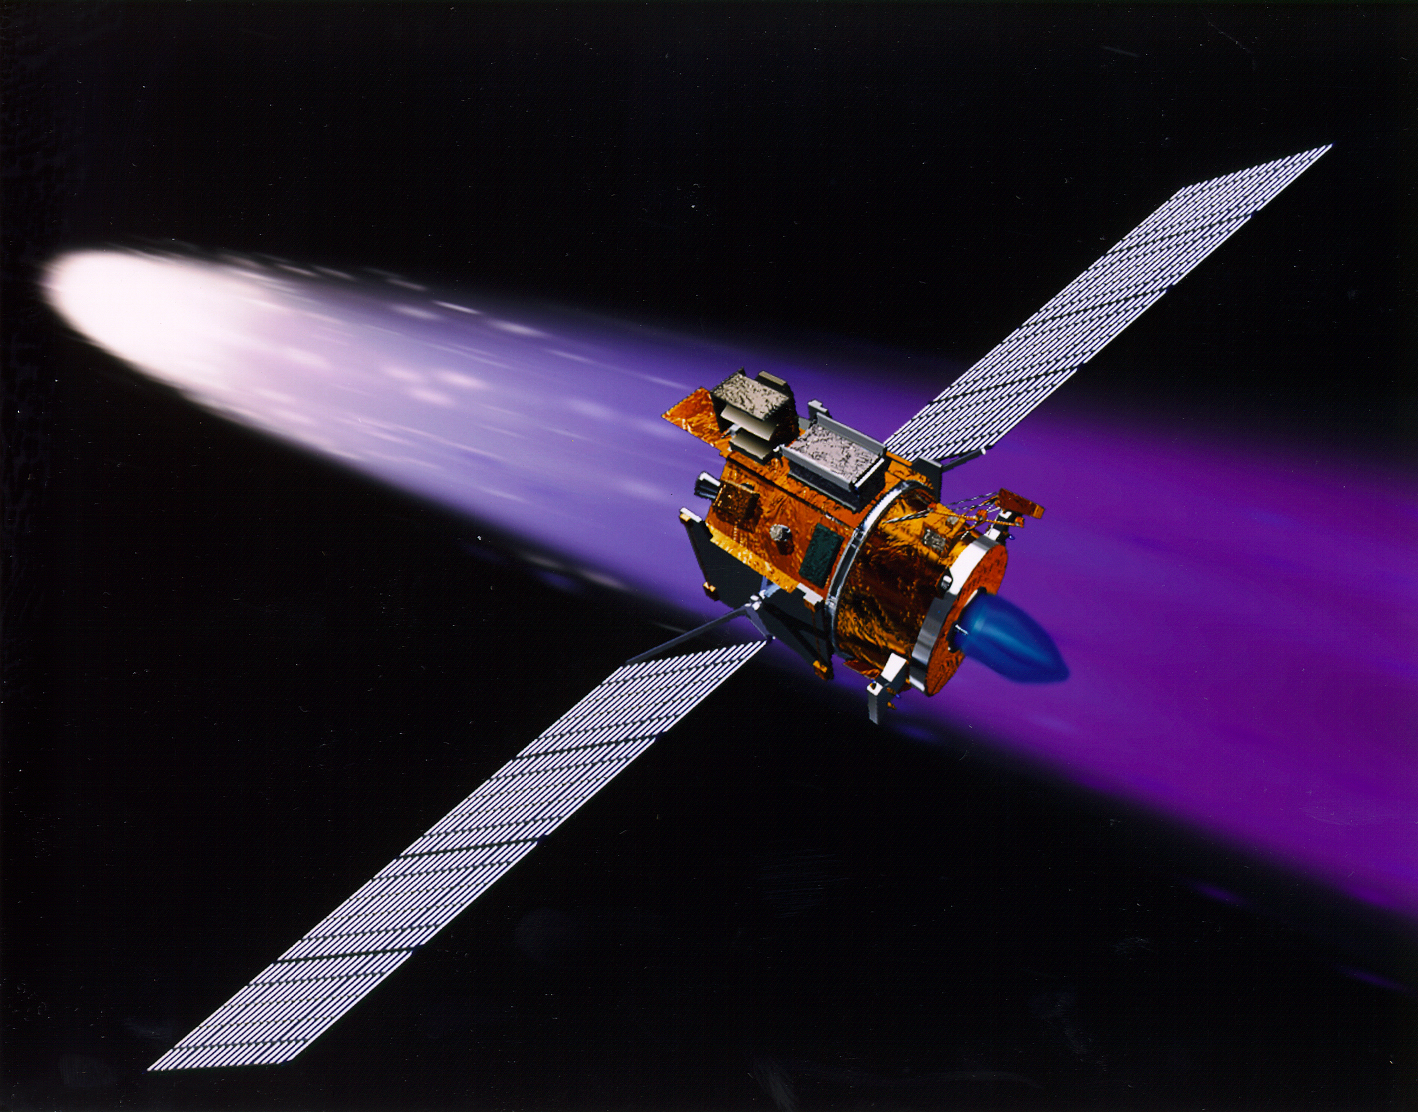
\includegraphics[height=0.4\textheight,width=0.5\textwidth,keepaspectratio]{figures/defense/deepspace1.jpg}
\end{center}
\hyperlink{slide:propulsion}{\beamergotobutton{Ideal Rockets}}
\end{frame}   %-----------------------------%

\begin{frame}{Low Thrust Orbital Transfers} % -----------------------------------%
    \begin{itemize}
        \item Low Thrust orbital transfers using reachability sets 
        \begin{itemize}
            \item Transfer design on lower dimensional \Poincare surface
            \item Simple method to incorporate effects of low-thrust 
            \item Avoids the issue of determining initial conditions
        \end{itemize}
    \pause
        \item Alleviates many issues with previous approaches
        \begin{itemize}
            \item Initial states chosen from from the reachable set
            \item Indirect optimal control vs. direct optimal control
            \item Reachability set gives bounds on motion
        \end{itemize}    
    \end{itemize}

  \note[itemize]{
    \item here we introduce some of our previous work that aims to apply geometric mechanics to the design of trajectories around asteroids
    \item Reachability set avoids the need to pick initial conditions
    \item We compute on a lower dimensional surface
  }
\end{frame} %--------------------------------------%

\subsubsection[Dynamic Systems Theory Review]{Dynamic Systems}

\begin{frame}{\Poincare map}
\begin{itemize}
    \item Intersection of a periodic orbit with a lower dimensional subspace
    \pause
        \begin{itemize}
            \item  \Emph{\Poincare section} - discrete map between intersections
        \end{itemize}
        \pause
    \item Useful for investigating the stability and structure 
    \pause
    \item Define a \Poincare section \( \Sigma \) 
        \begin{itemize}
            \item Used for initial and target periodic orbits
            \item Subspace for the \Emph{reachability set}
        \end{itemize}
\end{itemize}

\begin{center}
    \resizebox{!}{0.5\textheight}{%
        \tikzsetnextfilename{poincare_map}
\tdplotsetmaincoords{60}{125} % view angle in spherical coordinates
\begin{tikzpicture}[
    tdplot_main_coords, 
    poincare/.style={opacity=.2,
    very thick,
    fill=blue},
    orbit/.style={very thick,black},
    orbit hidden/.style={very thick,dashed}, 
    grid/.style={very thin,gray!50},
    axis/.style={->,blue,thick},
    ]

    % nodes for the poincare section
    \node[label=above:\(\Sigma\)] (upper_right) at (0,5,5) {}; 
    \node[] (upper_left) at (0,1,5) {}; 
    \node[] (lower_left) at (0,1,0) {};
    \node[] (lower_right) at (0,5,0) {};

        % draw poincare section
    \draw[poincare] (upper_right.center) -- (upper_left.center) --
        (lower_left.center) -- (lower_right.center) --
        (upper_right.center);

        % draw a periodic orbit
    \coordinate (center) at (0,0,2); 
    \node[below right] (x0) at (0,2,2) {\(\vecbf{q}_0\)}; 
    \filldraw (0,2,2) circle (3pt);

    \node[below right] (x1) at (0,3,2) {\(\vecbf{q}_1\)};
    \filldraw (0,3,2) circle (3pt);

    \tdplotdrawarc[orbit hidden]{(center)}{2}{90}{190}{}{};
    \tdplotdrawarc[orbit,<-]{(center)}{2}{-170}{90}{}{};

    \tdplotdrawarc[orbit hidden]{(center)}{3}{90}{199}{}{};
    \tdplotdrawarc[orbit,<-]{(center)}{3}{-161}{90}{}{};

\end{tikzpicture}

    }
\end{center}

\note[itemize]{
    \item Here we present a review of the key components of dynamical systems theory
    \item we start with some initial condition \( {x}_0\) on a periodic orbit
    \item we then define a section \( \Sigma \) transverse to this flow
    \item we can use the successive iterations of these periodic orbits to study the dynamics of the system on a lower dimensional surface.
    \item Periodic orbits show up as fixed points while sinks/sources will have a distinctly different behavior
}
\end{frame}

\begin{frame}{Reachability Set}

\begin{itemize}
    \item Set of states achievable from a given initial condition over fixed \( t_f \) s.t. maximum control constraint
    \[
        R( \vc{x}_0, \mathcal{U} , t_f) = \braces{ \vc{x}_f \subseteq \mathcal{X} | \exists \vc{u} \in \mathcal{U}, \vc{x}(t_f) = \vc{x}_f }
    \]
    \pause
    \item Directly derivable from optimal control
    \item Frequently used for safety planning, e.g. air traffic avoidance
    \item We extend to the design of orbital transfers
\end{itemize}

\note[itemize]{
    \item Given the state of an aircraft, we can predict where it can end up over a fixed amount of time.
    \item To avoid any possibility of collision, we want to make sure these sets do not intersect
}
\end{frame}

\begin{frame}{Low Thrust Transfers via Reachability Sets } % -----------------------------------%

\begin{itemize}
    \item Generate the reachability set on a \Poincare section, \( \Sigma \)
    \item Control input is chosen to enlarge the reachable set
\end{itemize}

\begin{center}
    \resizebox{!}{0.8\textheight}{%
        \tdplotsetmaincoords{60}{125} % view angle in spherical coordinates
\begin{tikzpicture}[
    tdplot_main_coords,
    poincare/.style={opacity=.2,very thick,fill=blue},
    orbit/.style={very thick,black},
    orbit hidden/.style={very thick,dashed},
    grid/.style={very thin,black},
    axis/.style={->,blue,thick},
    reachability/.style={thick,blue},
    ]

        % nodes for the poincare section
    \node[label=above:\(\Sigma\)] (upper_right) at (0,5,5) {};
    \node[] (upper_left) at (0,1,5) {};
    \node[] (lower_left) at (0,1,0) {};
    \node[] (lower_right) at (0,5,0) {};

    % draw poincare section
    \draw[poincare] (upper_right.center) -- (upper_left.center) -- (lower_left.center) -- (lower_right.center) -- (upper_right.center);
    
    % draw a periodic orbit
    \coordinate (center) at (0,0,2);
    \node[label=below:\(\vecbf{x}_n\)] (x0) at (0,3,2) {};
    % \node[label=below:\(\vecbf{x}_n\)] at (x0) {};
    \filldraw (x0) circle (3pt);

    % \tdplotdrawarc[orbit hidden]{(center)}{3}{90}{200}{}{};
    \tdplotdrawarc[orbit,<-]{(center)}{3}{-160}{90}{}{};

    % draw reachability set on the poincare section
    \coordinate (reach) at (0,4.5,2);
    \tdplotsetthetaplanecoords{90}

    \draw[tdplot_rotated_coords,grid] (x0) -- (reach);
    \draw[tdplot_rotated_coords,grid] (x0) -- ++(-45:1.5);

    \tdplotdrawarc[tdplot_rotated_coords,grid]{(x0)}{0.5}{-45}{90}{above}{\(\theta_d\)};

    % draw terminal state on reachability set
    \node[tdplot_rotated_coords,label=above:\(\vecbf{x}_f\)] (xf) at ($ (x0)+(-45:1.5) $) {};
    \filldraw (xf) circle (3pt);

    \node[tdplot_rotated_coords,label=below:\(J\)] at (xf) {};

    \tdplotdrawarc[tdplot_rotated_coords,reachability]{(x0)}{1.5}{0}{360}{}{};
        % place
\end{tikzpicture}

    }
\end{center}

\note[itemize]{
    \item We combine both reachability and the \Poincare section to design transfers
    \item again we define our section \( \Sigma\)
    \item choose an initial state that is on \( \Sigma \)
    \item propogate without any control input from \( \vc{x}_0 \) to \( \vc{x}_n\)
    \item by adding the control input the terminal state will be something different at \( \vc{x}_f\)
    \item we define the distance between \( \vc{x}_n\) and \(\vc{x}_f\) with \( J \) - want to maximize this
    \item Repeat this computation many times for a variety of angles \( \phi\)
}
\end{frame} %--------------------------------------%

% show results of the transfer
\begin{frame}{Periodic Orbit Transfer}
    \begin{itemize}
        \item Transfer from periodic orbit to the Moon
        \item Orbit would provide constant line of site between Earth and far side
    \end{itemize}
    \begin{center}
        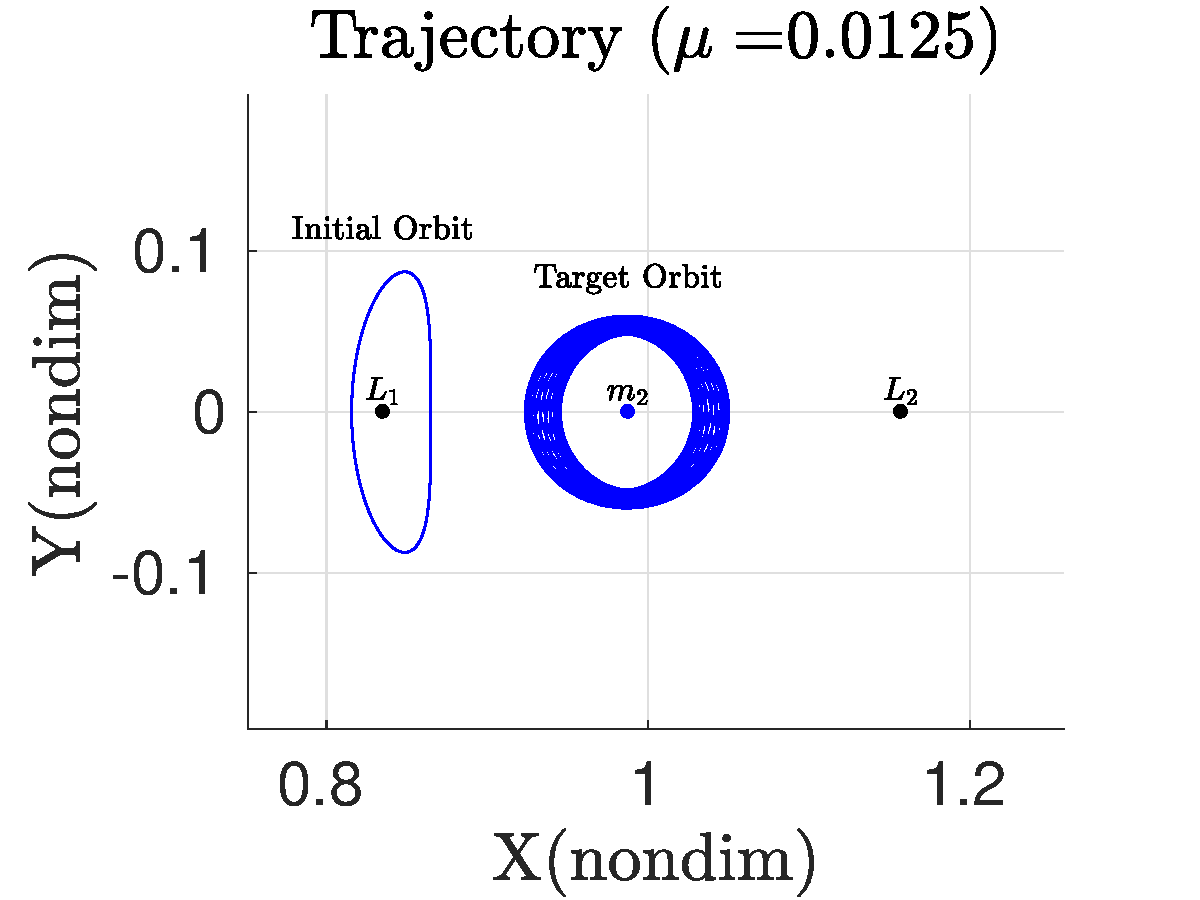
\includegraphics[height=0.75\textheight,keepaspectratio]{figures/2017_JAS/moon_orbit.pdf} % requires the graphicx package
   \end{center}
\end{frame}

\begin{frame}{Periodic Orbit Transfer}
    \begin{itemize}
        \item Reachable set is determined on the \Poincare section
        \item Intersection is used to determine the transfer
    \end{itemize}
    \begin{center}
        \only<1>{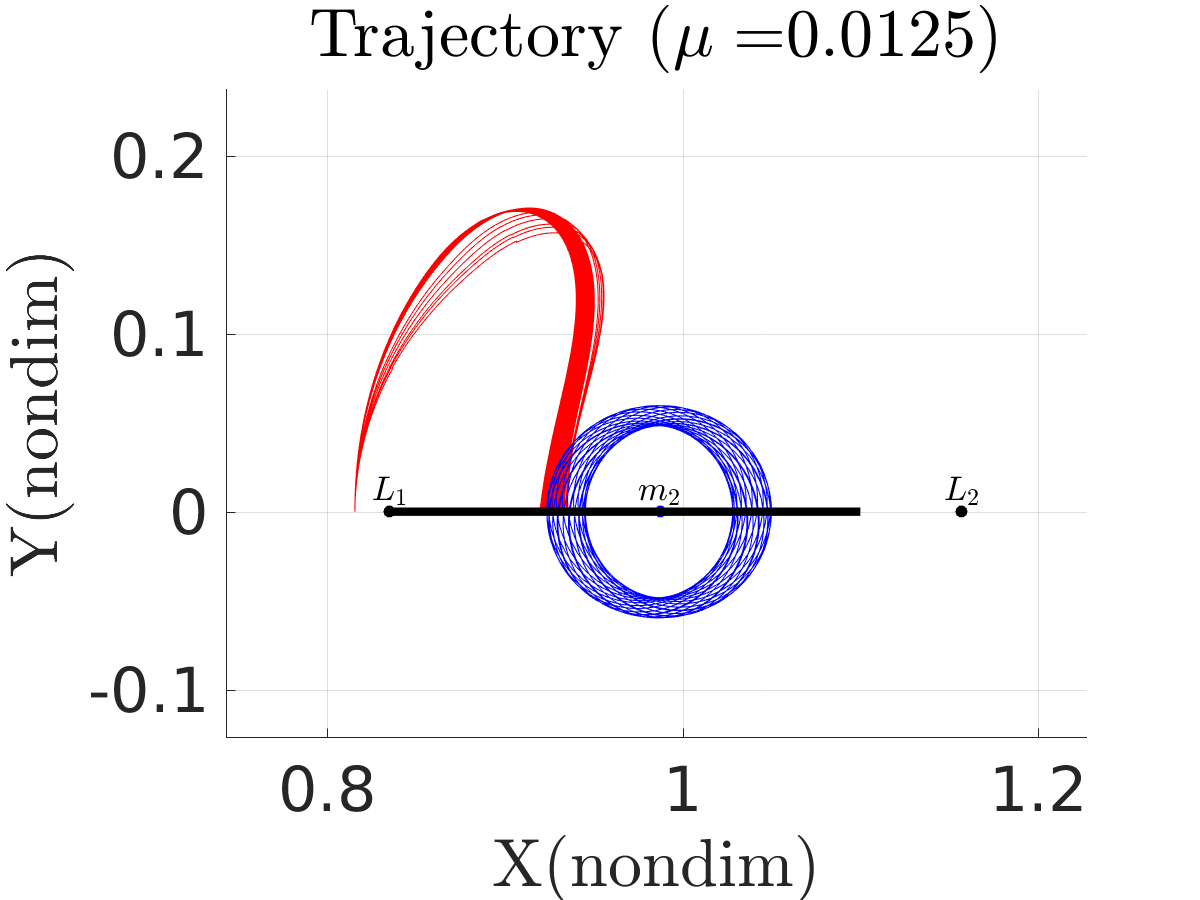
\includegraphics[width=0.5\textwidth]{figures/2017_JAS/reach_trajectory}}~
        \only<2>{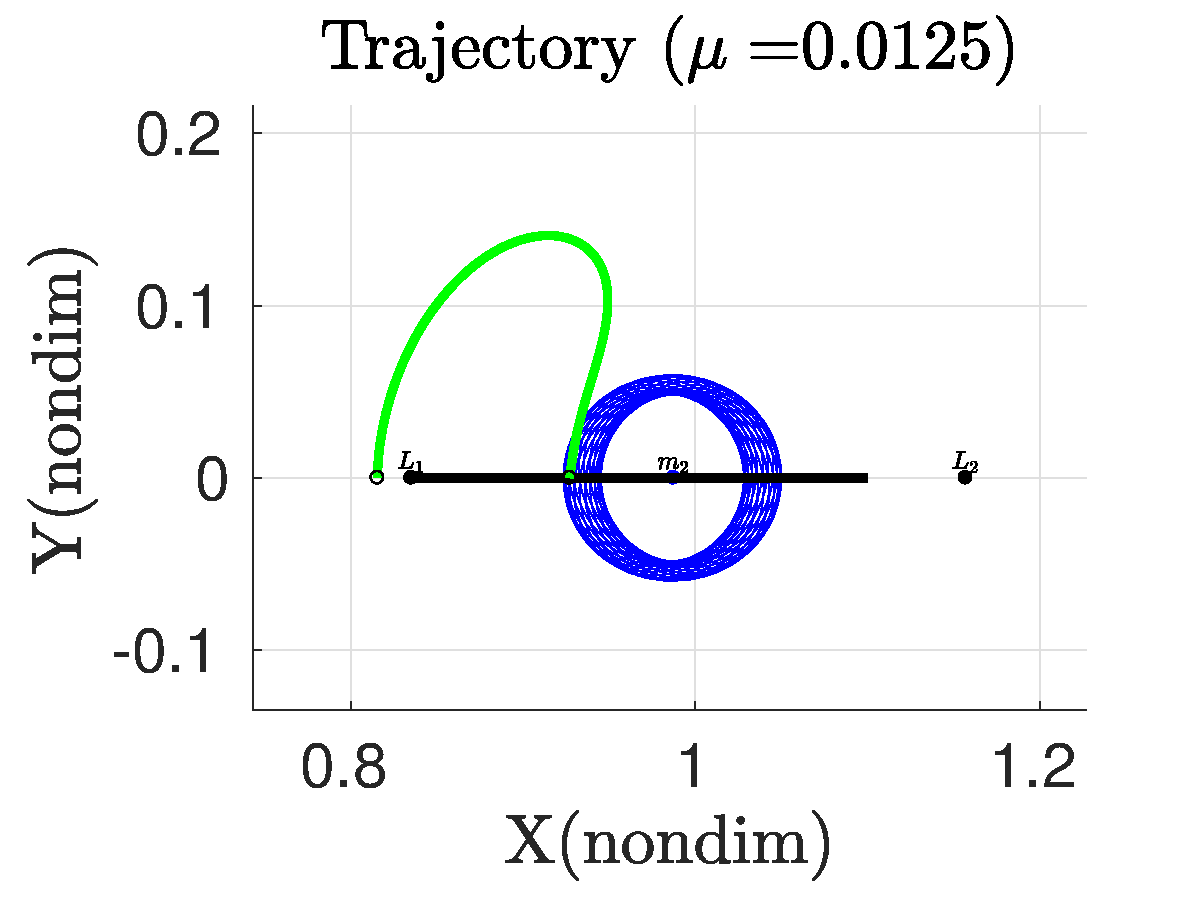
\includegraphics[width=0.5\textwidth]{figures/2017_JAS/reach_transfer.pdf}}~
        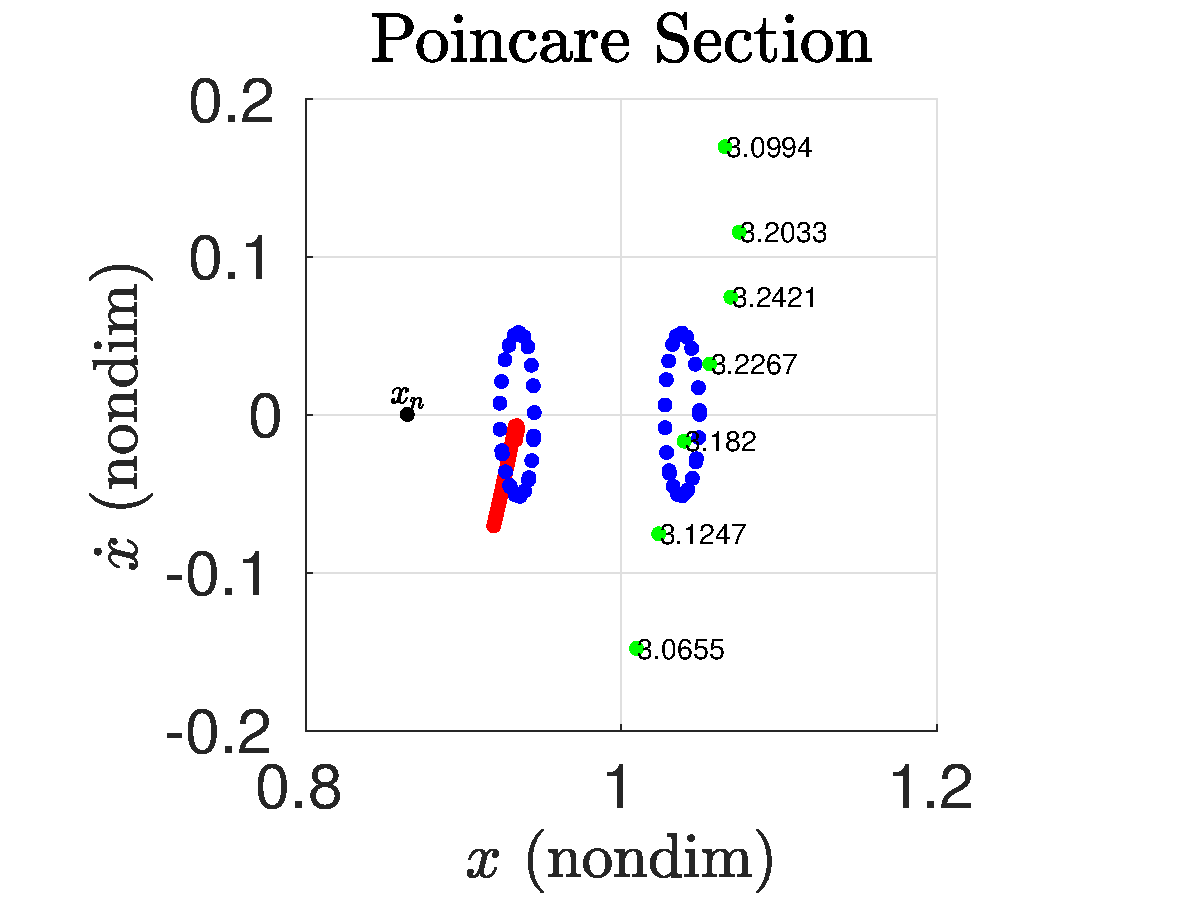
\includegraphics[width=0.5\textwidth]{figures/2017_JAS/poincare_compare} 
    \end{center}
\end{frame}

\begin{frame}{Geostationary Orbit Transfer}
    \begin{itemize}
        \item Now multiple reachable sets are combined for a larger transfer
        \item Transfer from geostationary to \( L_1 \) stable manifold
    \end{itemize}
    \begin{center}
            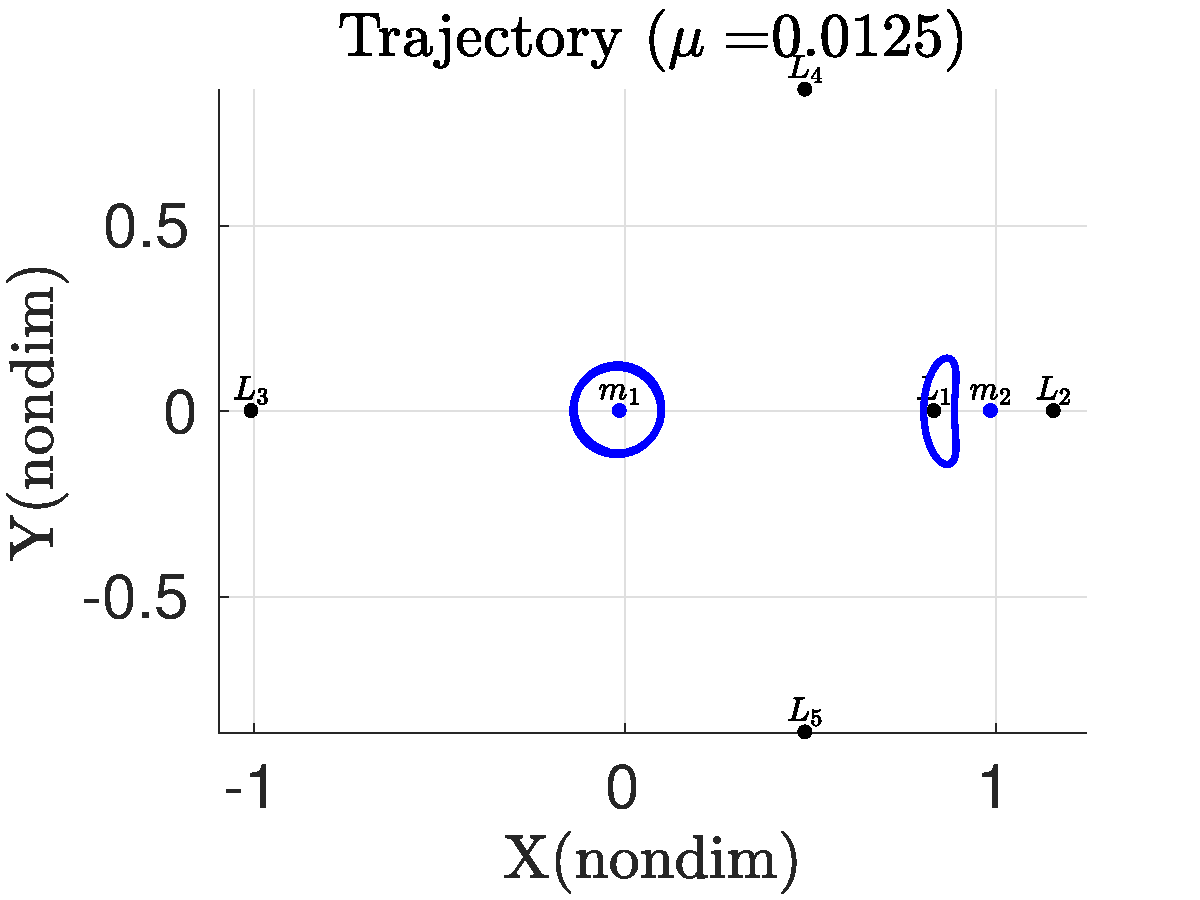
\includegraphics[height=0.8\textheight]{figures/2017_JAS/initial_final} % requires the graphicx package
    \end{center}
\end{frame}

\begin{frame}{Geostationary Orbit Transfer}
    \begin{itemize}
        \item Multiple reachability sets are linked to generate a transfer
    \end{itemize}
    \begin{center}
        \only<1>{
        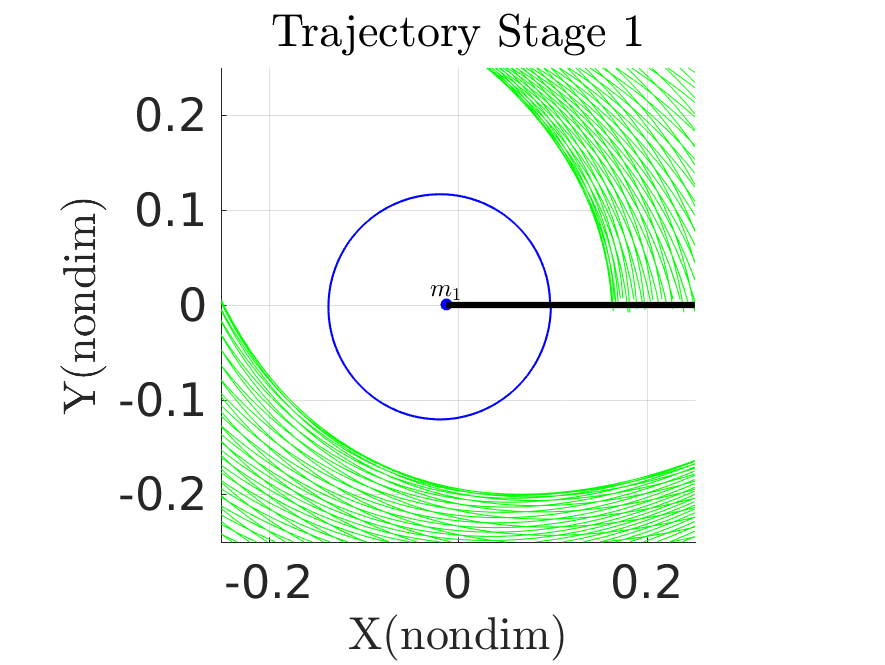
\includegraphics[height=0.8\textheight,width=0.5\textwidth,keepaspectratio]{figures/2017_JAS/stage1_trajectory_zoom.pdf}~
        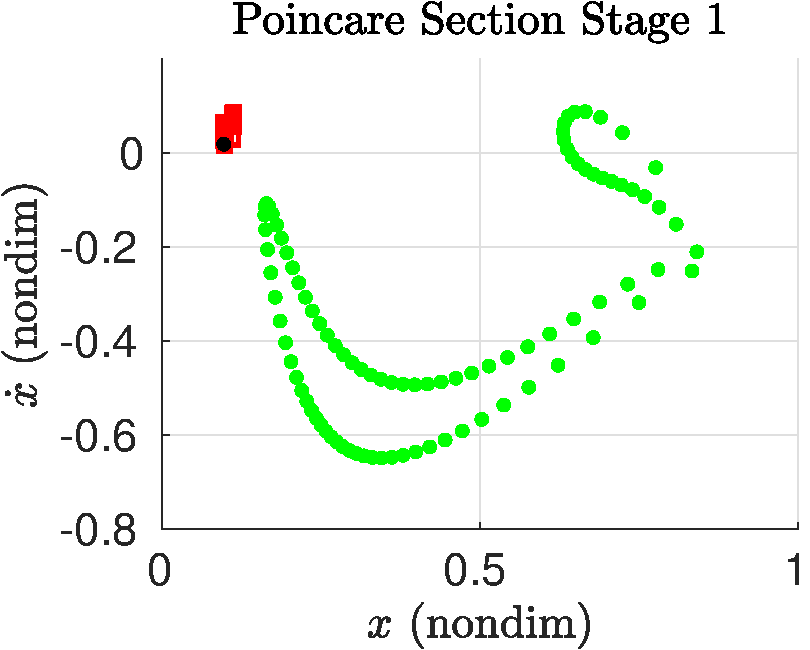
\includegraphics[height=0.8\textheight,width=0.5\textwidth,keepaspectratio]{figures/2017_JAS/stage1_poincare.pdf}
    }
        \only<2>{
        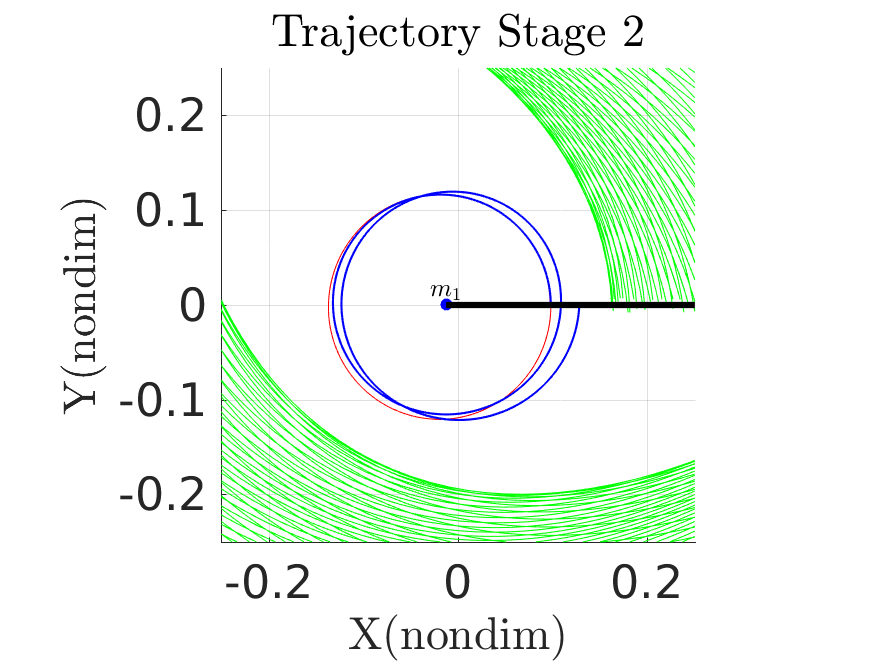
\includegraphics[height=0.8\textheight,width=0.5\textwidth,keepaspectratio]{figures/2017_JAS/stage2_trajectory_zoom.pdf}~
        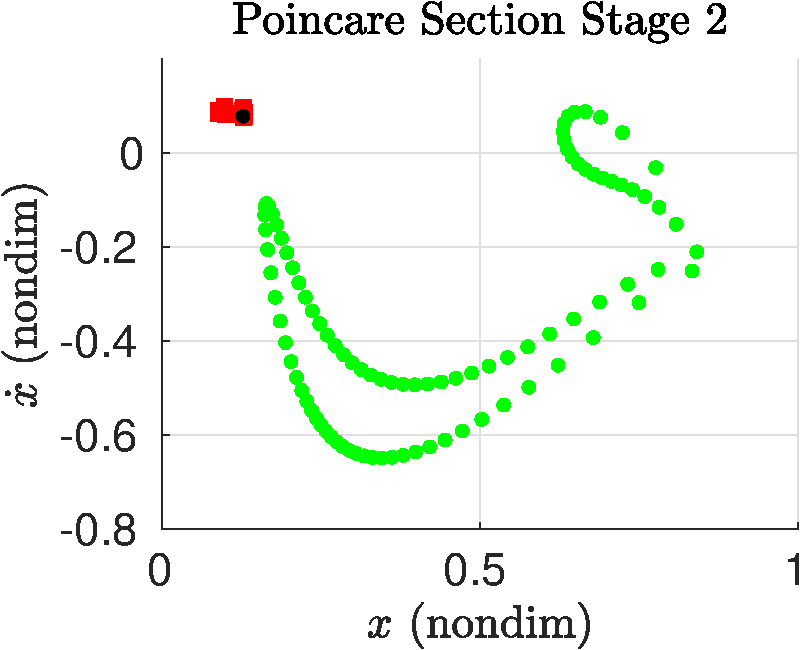
\includegraphics[height=0.8\textheight,width=0.5\textwidth,keepaspectratio]{figures/2017_JAS/stage2_poincare.pdf}
    }
        \only<3>{
        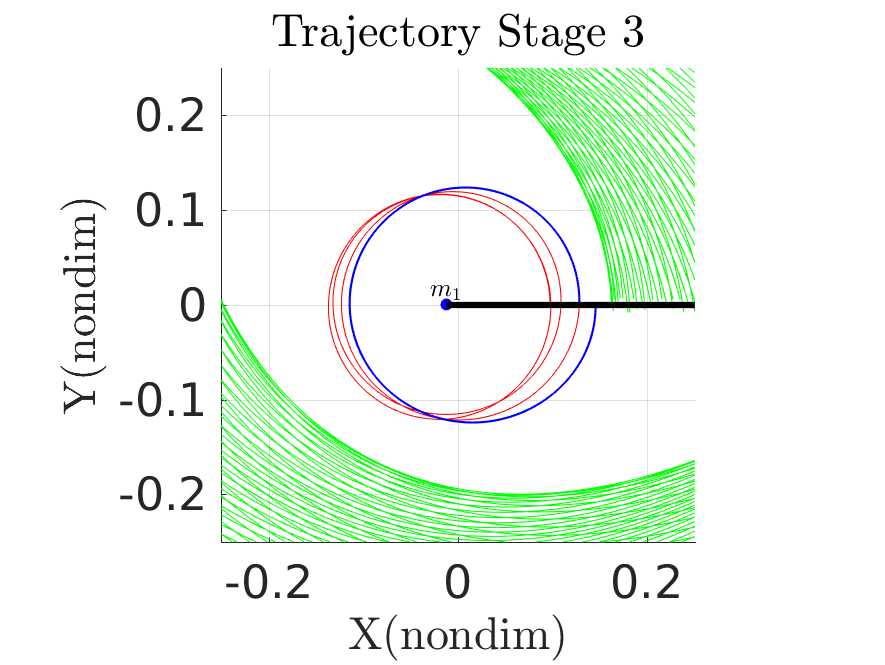
\includegraphics[height=0.8\textheight,width=0.5\textwidth,keepaspectratio]{figures/2017_JAS/stage3_trajectory_zoom.pdf}~
        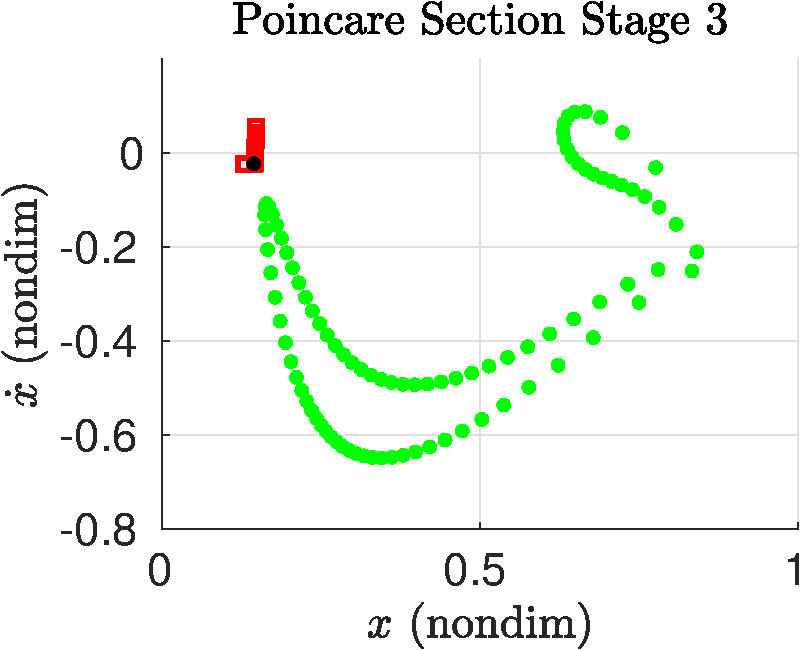
\includegraphics[height=0.8\textheight,width=0.5\textwidth,keepaspectratio]{figures/2017_JAS/stage3_poincare.pdf}
    }
        \only<4>{
        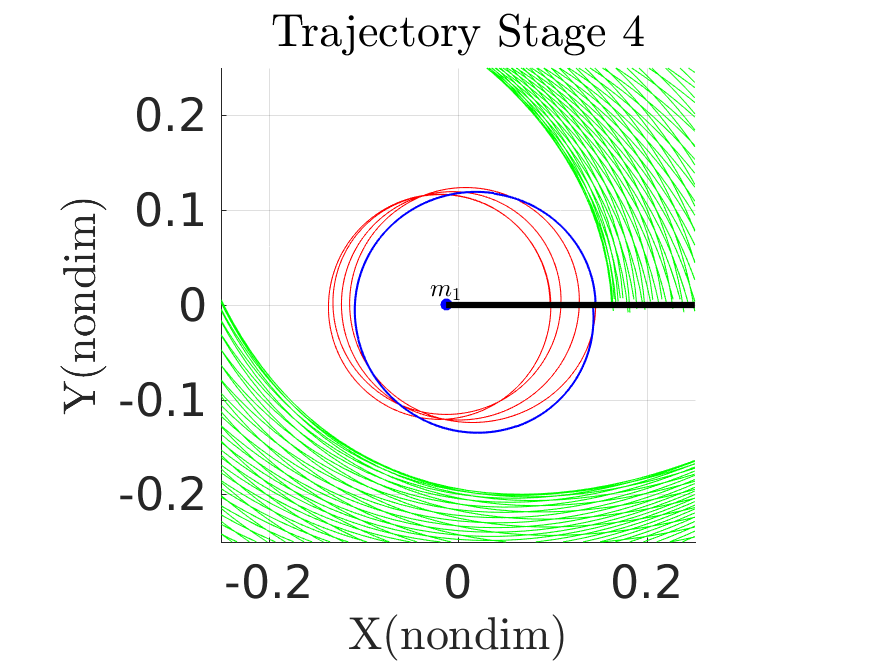
\includegraphics[height=0.8\textheight,width=0.5\textwidth,keepaspectratio]{figures/2017_JAS/stage4_trajectory_zoom.pdf}~
        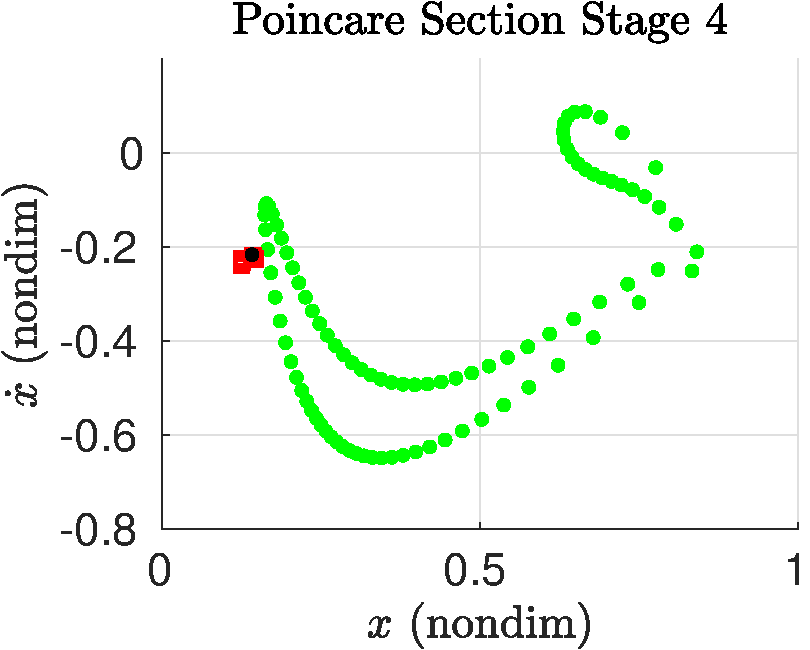
\includegraphics[height=0.8\textheight,width=0.5\textwidth,keepaspectratio]{figures/2017_JAS/stage4_poincare.pdf}
    }
        \only<5>{
        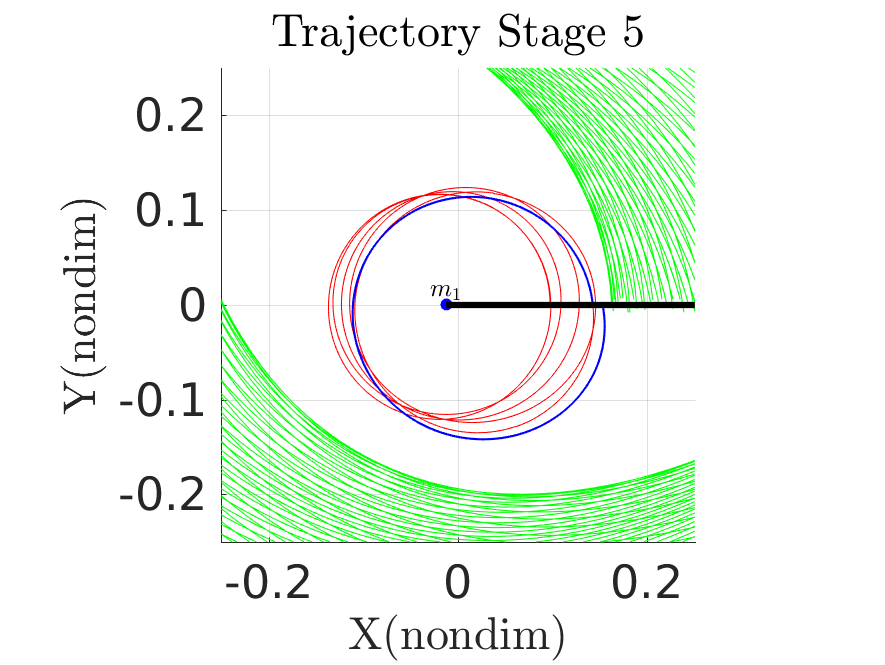
\includegraphics[height=0.8\textheight,width=0.5\textwidth,keepaspectratio]{figures/2017_JAS/stage5_trajectory_zoom.pdf}~
        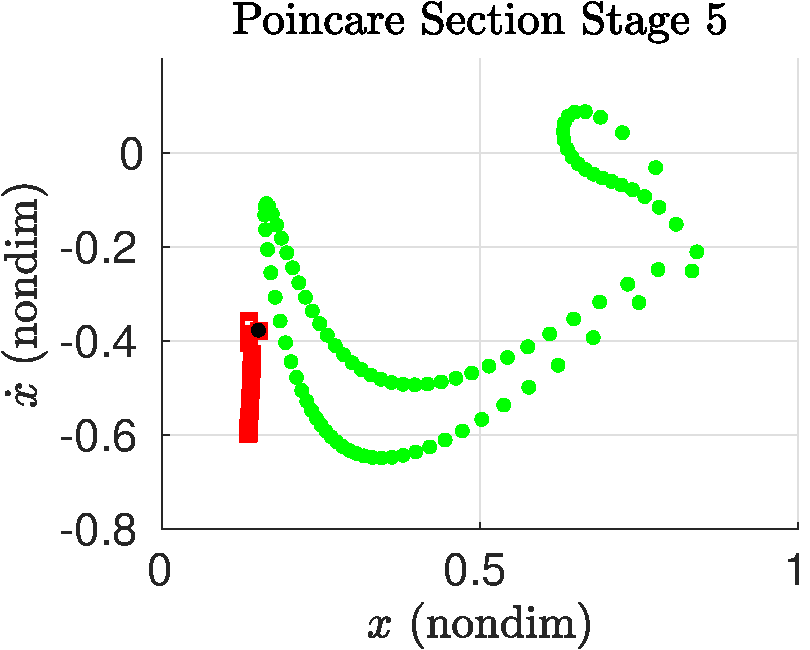
\includegraphics[height=0.8\textheight,width=0.5\textwidth,keepaspectratio]{figures/2017_JAS/stage5_poincare.pdf}
    }
        \only<6>{
        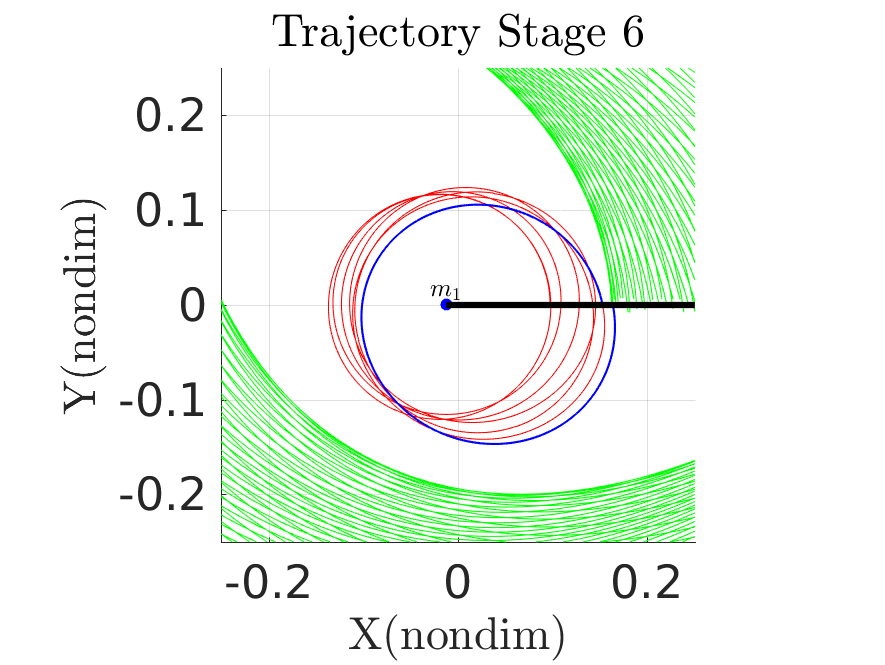
\includegraphics[height=0.8\textheight,width=0.5\textwidth,keepaspectratio]{figures/2017_JAS/stage6_trajectory_zoom.pdf}~
        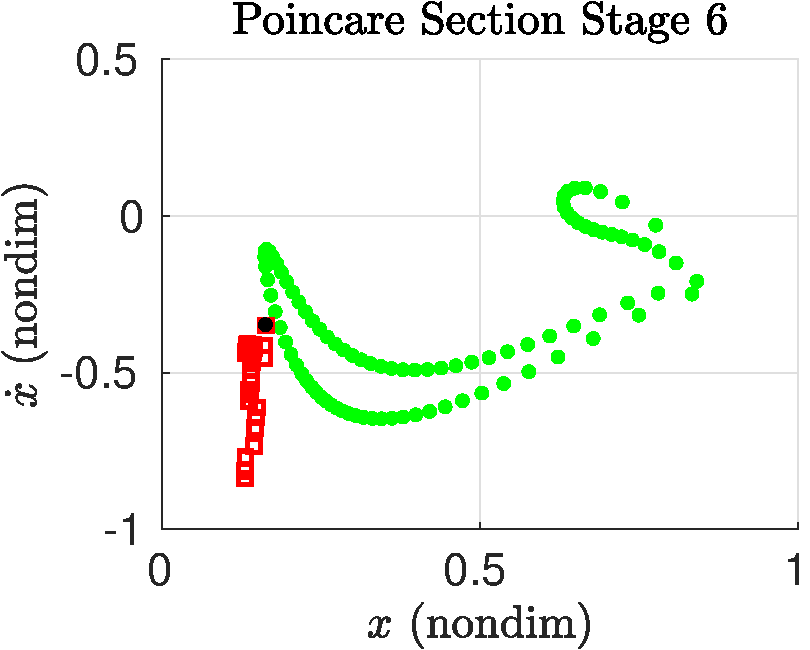
\includegraphics[height=0.8\textheight,width=0.5\textwidth,keepaspectratio]{figures/2017_JAS/stage6_poincare.pdf}
    }
        \only<7>{
        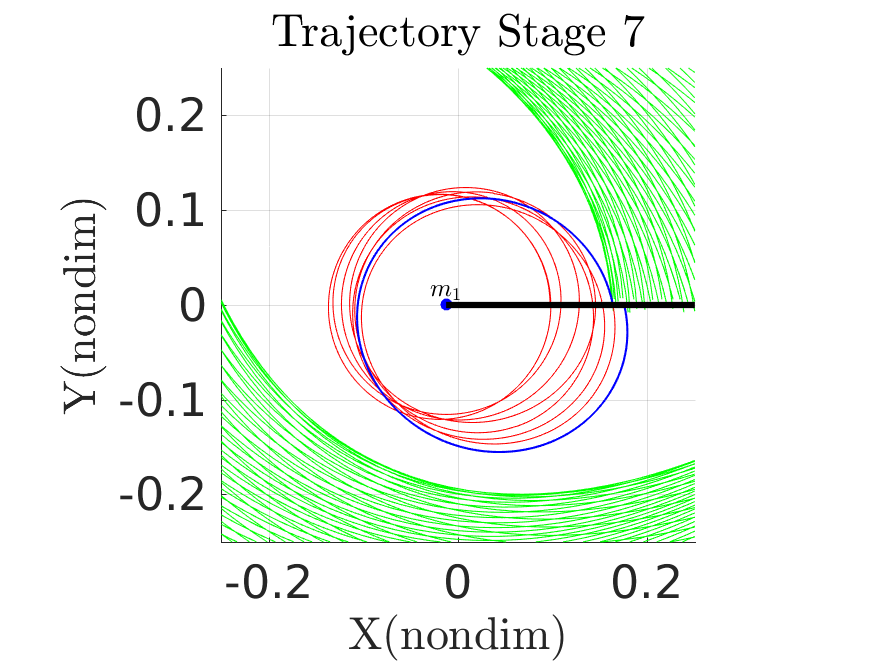
\includegraphics[height=0.8\textheight,width=0.5\textwidth,keepaspectratio]{figures/2017_JAS/stage7_trajectory_zoom.pdf}~
        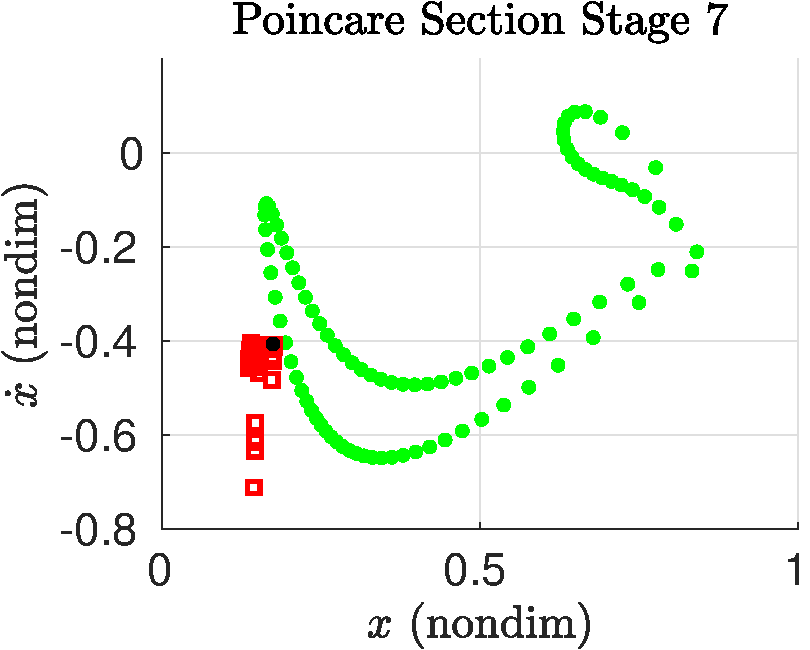
\includegraphics[height=0.8\textheight,width=0.5\textwidth,keepaspectratio]{figures/2017_JAS/stage7_poincare.pdf}
    }
        \only<8>{
        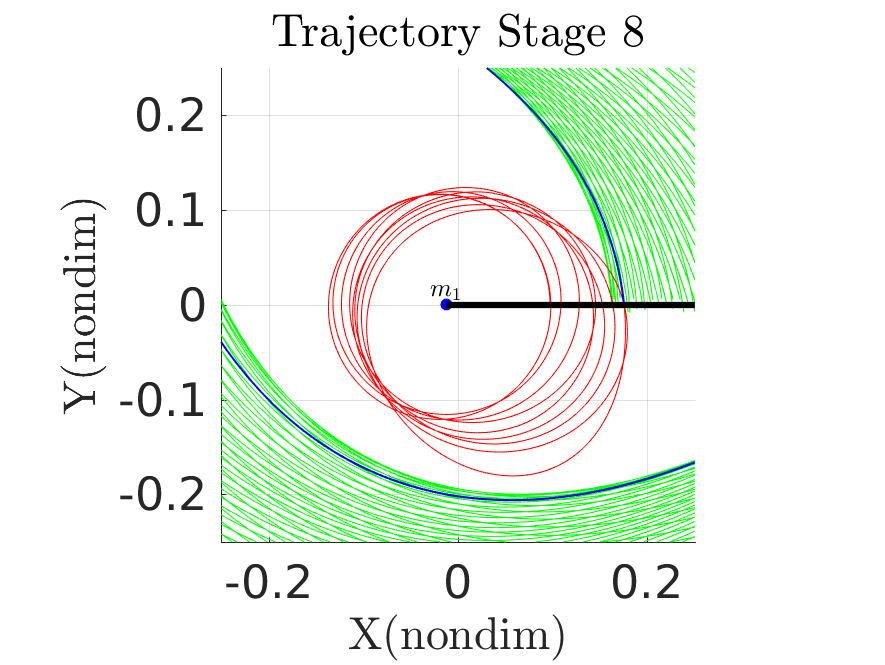
\includegraphics[height=0.8\textheight,width=0.5\textwidth,keepaspectratio]{figures/2017_JAS/stage8_trajectory_zoom.pdf}~
        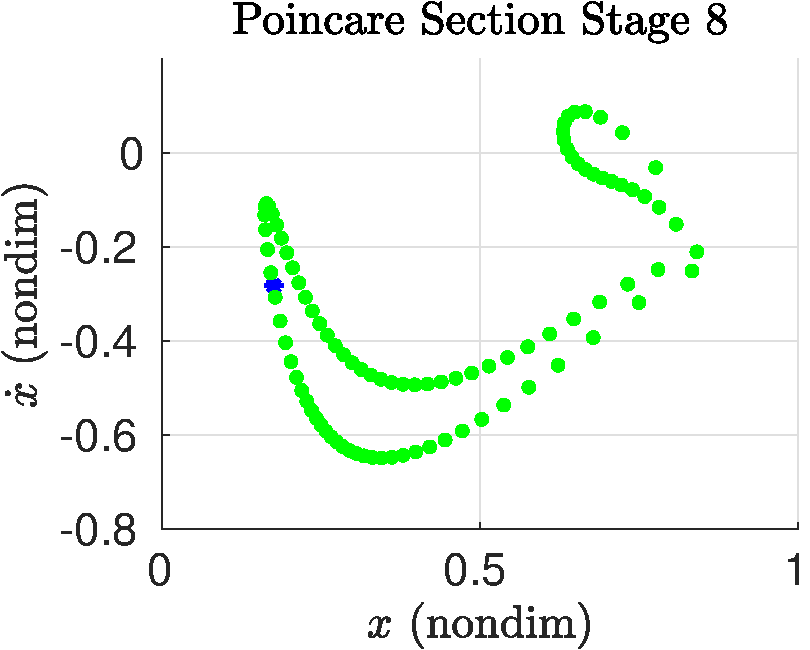
\includegraphics[height=0.8\textheight,width=0.5\textwidth,keepaspectratio]{figures/2017_JAS/stage8_poincare.pdf}
    }
    \only<9>{
        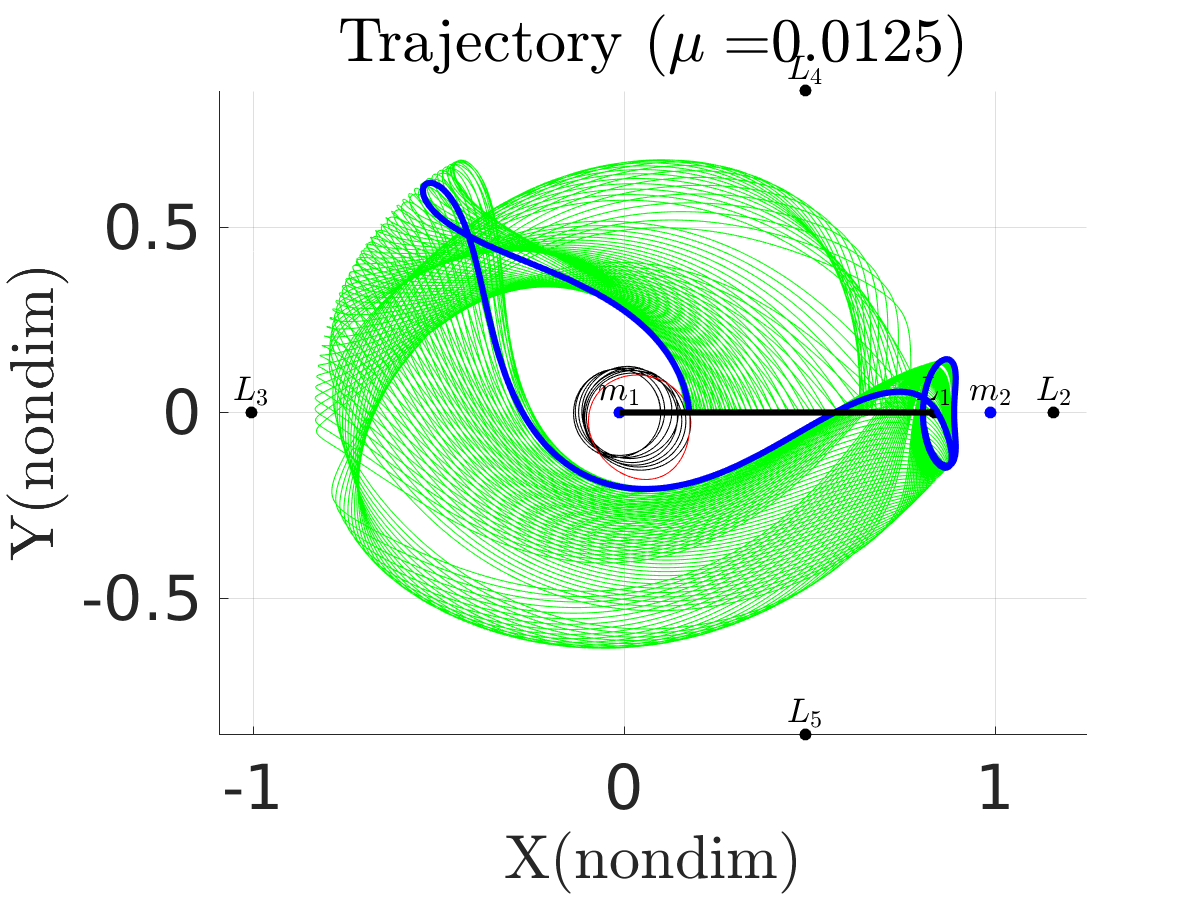
\includegraphics[width=0.45\textwidth]{figures/2017_JAS/geo_transfer_full}~
        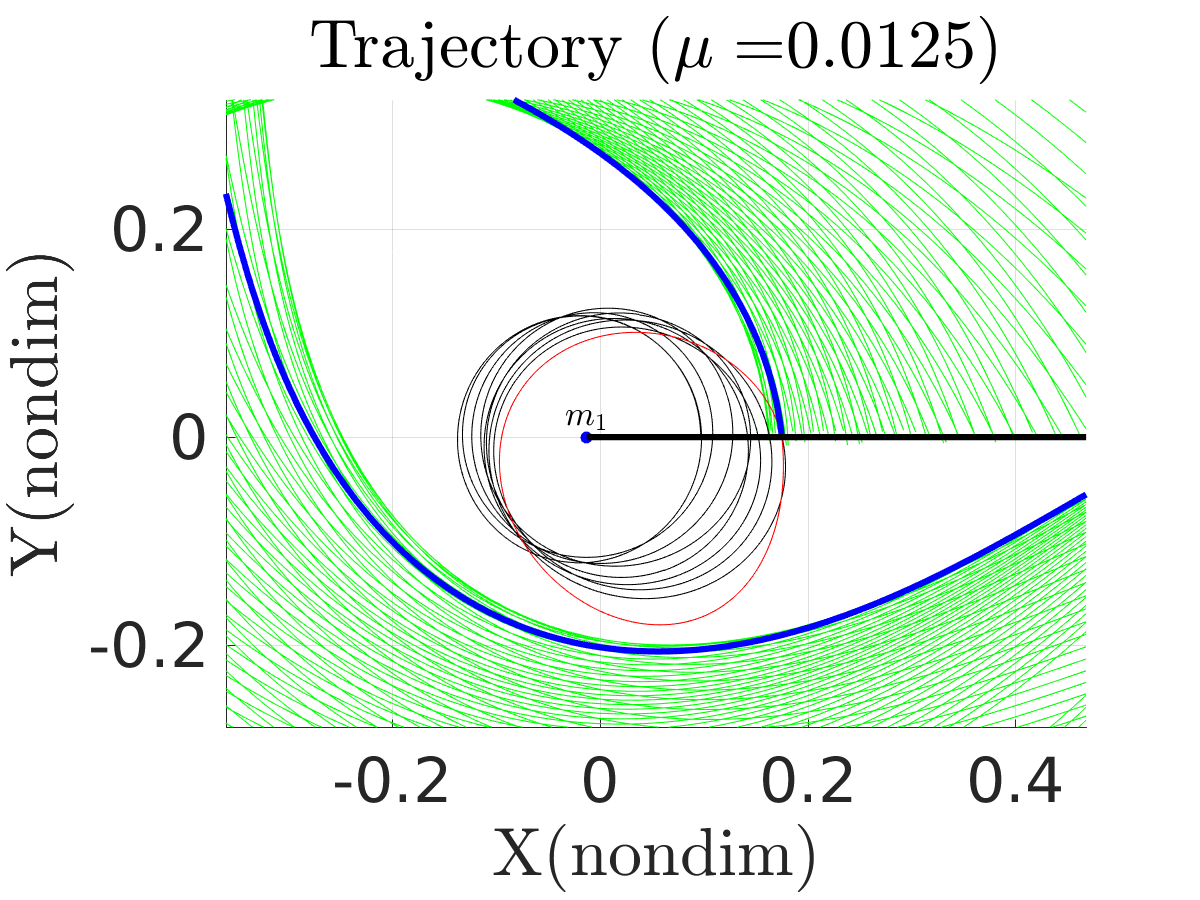
\includegraphics[width=0.45\textwidth]{figures/2017_JAS/geo_transfer_zoom}
    }
    \end{center}
\end{frame}

\begin{frame}{4769 Castalia Transfer}
    \begin{itemize}
        \item Extend the transfer to full 3D case around an asteroid
        \item Reachability set is now four dimensional
    \end{itemize}
    \begin{center}
        \only<1>{
        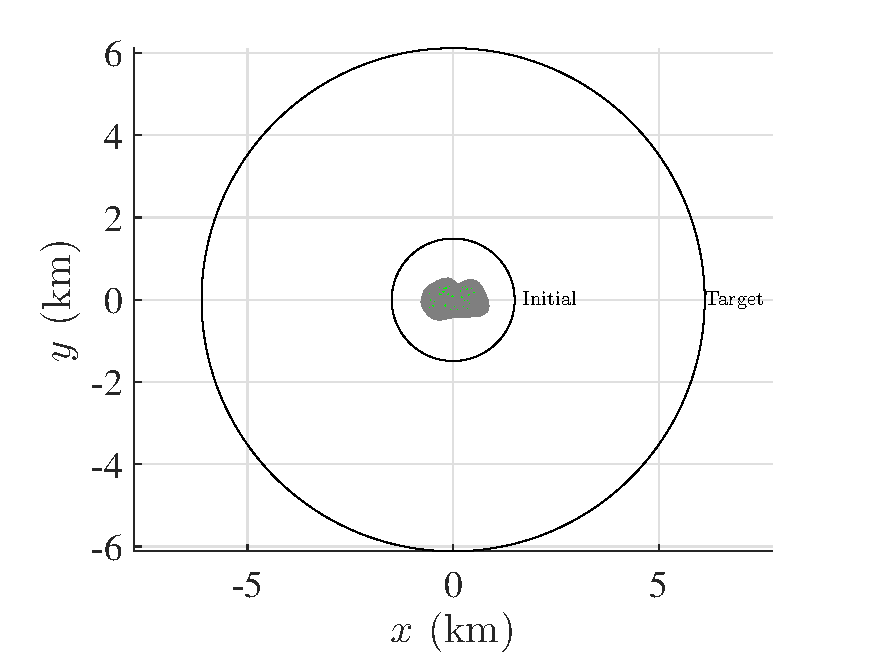
\includegraphics[width=0.5\textwidth]{figures/2016_AAS/initial_transfer}~
        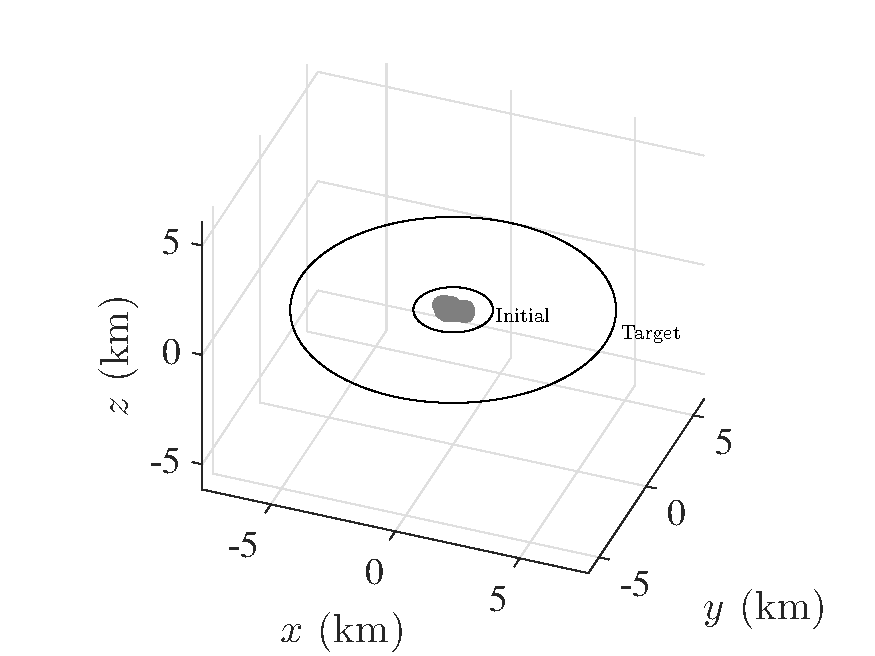
\includegraphics[width=0.5\textwidth]{figures/2016_AAS/initial_transfer_3d} 
    }
    \only<2>{
        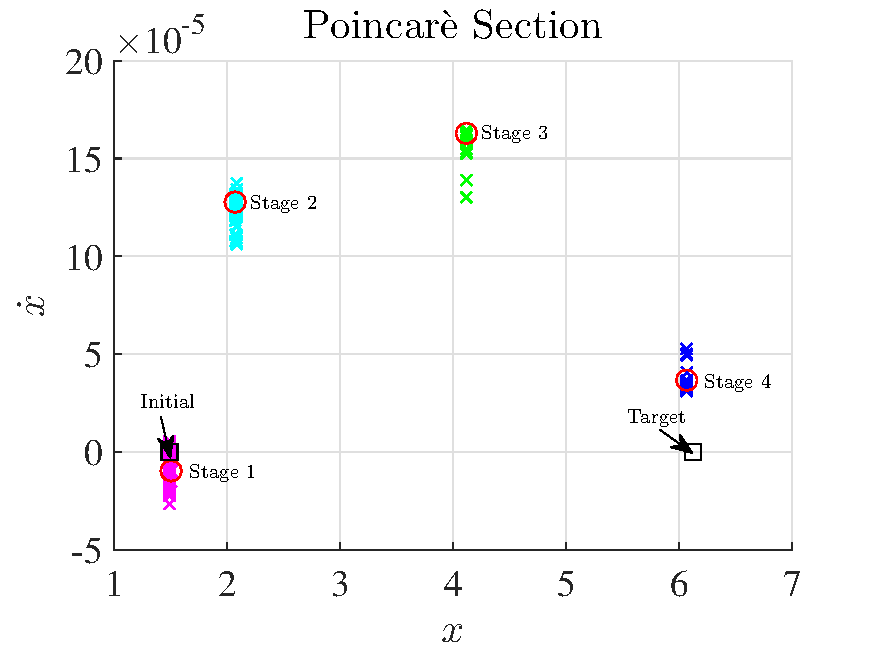
\includegraphics[width=0.5\textwidth]{figures/2016_AAS/poincare_xvsxdot.pdf}~
        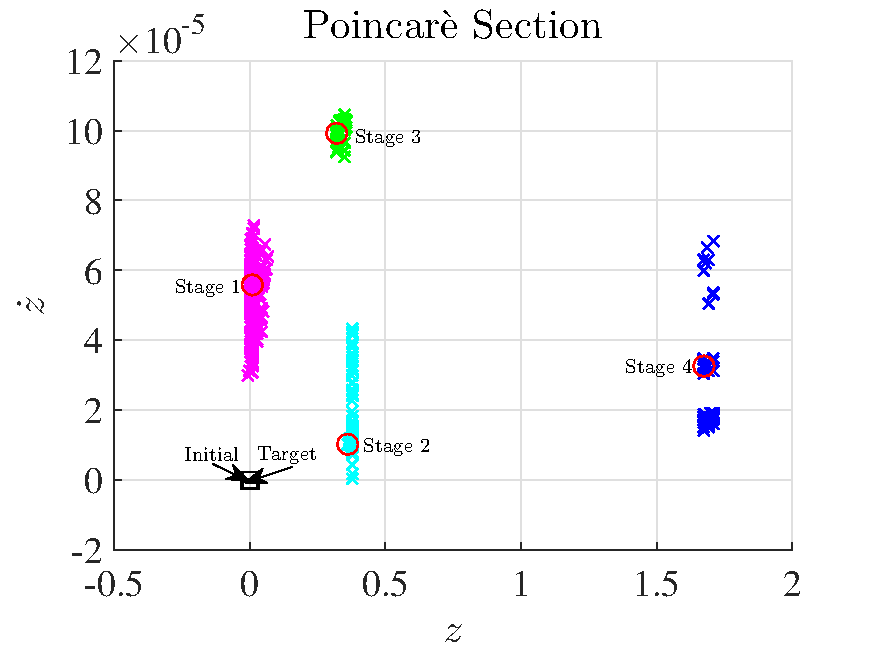
\includegraphics[width=0.5\textwidth]{figures/2016_AAS/poincare_zvszdot.pdf} 
    }
    \only<3>{
        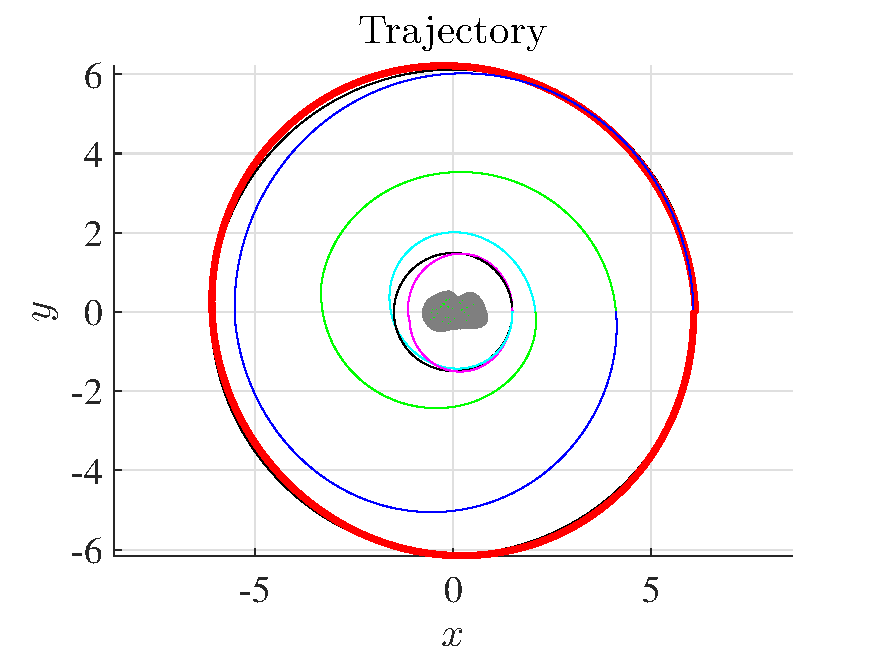
\includegraphics[width=0.5\textwidth]{figures/2016_AAS/trajectory.pdf}~
        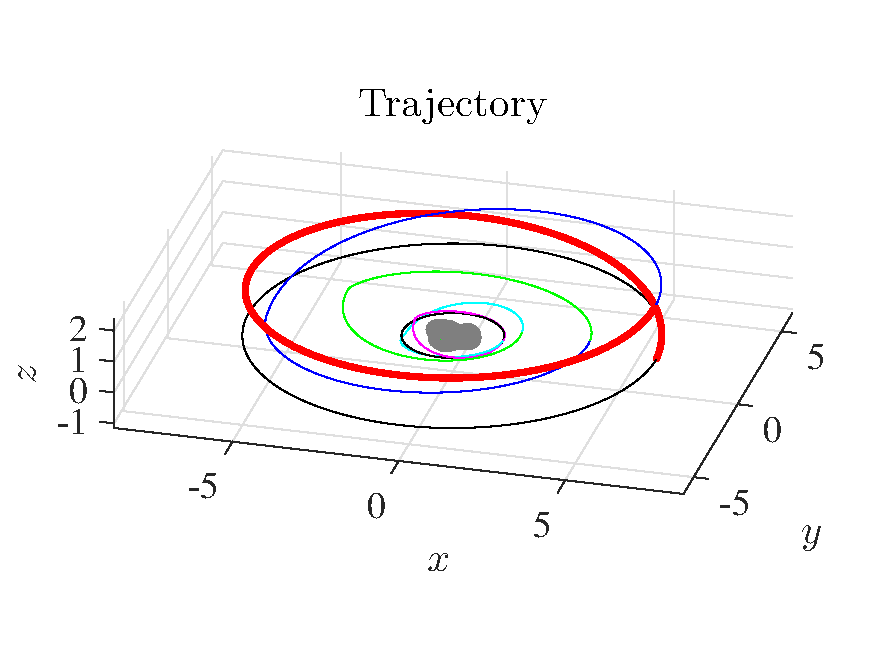
\includegraphics[width=0.5\textwidth]{figures/2016_AAS/trajectory_3d.pdf} 
    }
    \end{center}
\end{frame}
